\chapter{A! Foundations / Psi Implementationen}

... Psi has been implemented by different groups ...

\section{A! Psi Implementations}

\subsection{Dörners Implementation}

... Dörner implemented it in Pascal ...

\section{Joschas Implementation}

"The cognitive architecture MicroPsi builds on a framework for simulating agents as neuro-symbolic spreading activation networks. These agents are situated in a simulation environment or fitted with robotic bodies. The current implementation of MicroPsi has been re-implemented from the ground up and is described here."~\cite{conf/agi/Bach12}

\subsection{microPsi in Java}

"The first implementation of the MicroPsi framework spanned the years 2003 to 2009, and was built in Java as a set of plugins for the Eclipse IDE. The graphical edi- tor was built on SWT. It comprised about 60000 lines of code, and although a lot of effort went towards platform independence (with the exception of a DirectX/.Net based 3D viewer component), deployment on the various operating systems and across several versions of Eclipse became support intensive, especially after its adop- tion by teams outside of our group."~\cite{conf/agi/Bach12}

... Joscha implemented it in Java ...

\subsection{microPsi in Python}

"Gradual changes in the formalization of MicroPsi and the emergence of new soft- ware development methodologies and tool chains, especially the move from Java design patterns and XML tools towards lightweight and agile Python code, prompted a complete rewrite of the MicroPsi framework, starting in 2011. The following sec- tion describes the overall structure of the framework, followed by detailed definitions of the node net formalism and the structure of simulation worlds that enable running MicroPsi agents."~\cite{conf/agi/Bach12}

The MicroPsi 2 user interface is rendered completely inside a web browser and the simulation is deployed as a web application. The UI components are based upon HTML/Javascript and "and facilitates the communication between the browser based renderer and the agent simulator via JSON and JSON remote procedure calls. Rendering is supported by Twitter’s widget library Bootstrap (2012) and the Javascript library PaperJS (Lehni and Puckey, 2011)."~\cite{conf/agi/Bach12}

... then in Python with a Webinterface ...

\subsection{Module Overview / Architecture}
... it consists of a Core an a Server module with different threads running ...

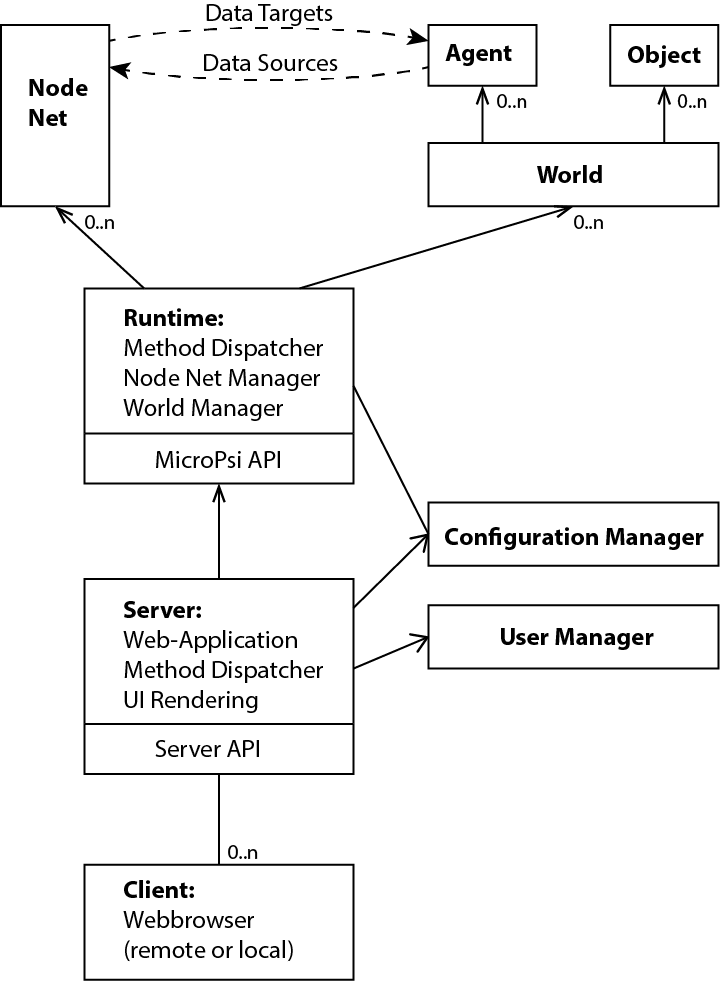
\includegraphics[width=5cm]{graphics/micropsi2_uml}

\subsection{Core}
... the core runs the heart of the simulation ...

\subsection{Server}
... the server provides the interface ...

\subsection{Simulation Environments}
... so far, there are an "Island" and an "Berlin" worlds ...

\section{A! Minecraft}
... a more complex simulation environment could be fun ...

... the story of Minecraft ...
... Minecrafts poularity (and demographics) ...

\subsection{What is Minecraft?}
... brief description of the basic mechanisms ...

\subsection{The Cient Server Protokoll}
... the language an external client needs to speak, to take place in a Minecraft world ...

\subsection{Suitability of Minecraft as a simulation environment}
... cheap licenses ...
... developer friendly community and game-studio ...
... sandbox game with many possibilieties but no pre-defined goals ...
... procedural semantic ...

\section{A! Minecraft and MicroPsi}
... a more complex simulation environment could be fun ...